\documentclass[11pt,a4paper]{article}
\usepackage[T1]{fontenc}
\usepackage[utf8]{inputenc}
\usepackage{babel}
\babelprovide[main,import]{french}
\usepackage[margin=23mm]{geometry}
\usepackage{amsmath,lmodern,microtype,booktabs,tabularx,array,graphicx,tikz,listings,xcolor,needspace}
\usetikzlibrary{arrows.meta,positioning}
\usepackage[pdfencoding=auto,colorlinks,linkcolor=blue!58!black,urlcolor=blue!58!black]{hyperref}
\graphicspath{{figures/}}
\definecolor{Encre}{HTML}{172A38}
\definecolor{Bleu}{HTML}{135776}
\definecolor{Papier}{HTML}{F0F5F7}
\color{Encre}
\lstset{basicstyle=\small\ttfamily,backgroundcolor=\color{Papier},columns=fullflexible,keepspaces=true,
  breaklines=true,showstringspaces=false,frame=none,aboveskip=8pt,belowskip=8pt}
\newcolumntype{Y}{>{\raggedright\arraybackslash}X}
\newcommand{\sel}[1]{\texttt{#1}}
\newcommand{\ui}[1]{\textsf{#1}}
\setlength{\parindent}{0pt}
\setlength{\parskip}{6pt}
\setlength{\emergencystretch}{3em}
\setcounter{tocdepth}{1}
\title{\bfseries Atelier SoSe\\\large Simulation, terrain et rejeu sur Pharo 14}
\author{}
\date{}

\begin{document}
\maketitle
\vspace{-1.6cm}
\noindent L'atelier exécute une simulation macro, calcule ses métriques et rejoue l'historique sur un terrain. SoSe et ISSe fournissent des références historiques. Les expériences paramétrées permettent de comparer les lois de commande, les hypothèses de perception et leurs effets sur la couverture.
{\small\setlength{\parskip}{0pt}\tableofcontents}

\clearpage
\part{Utiliser l'atelier}

\section{Préparer une première démonstration}
\begin{enumerate}
\item Lancez l'image avec le script livré, puis ouvrez \ui{Terrain et parcours}. Choisissez un site et cliquez sur \ui{Charger l'exemple}. Crozon se prête à un premier essai sur relief de côte. Les captures de Manhattan et Crozon ci-dessous ont été produites par le rendu natif.
\item Choisissez \ui{Parcours cartographié}, le nombre de drones et la durée du tik. Ce scénario reprend le tracé chargé. Cliquez sur \ui{Simuler} pour calculer l'historique.
\item Dans \ui{Affichage}, activez le parcours, les drones, la couverture et les masques. Choisissez le fond \ui{Relief ombré} ou \ui{Altitude} et vérifiez le cadrage avec \ui{Lire la carte}.
\item Dans \ui{Lecture}, choisissez la vitesse et la cadence d'échantillonnage. \ui{Exporter MP4…} enregistre les PNG, la chronologie \sel{lecture.ffconcat} et \sel{demonstration.mp4}.
\item Dans \ui{CSV}, cochez les métriques désirées puis exportez la série. Conservez les paramètres de mission et le dossier de terrain avec la vidéo si vous souhaitez la reproduire.
\end{enumerate}
\begin{figure}[ht]
\centering
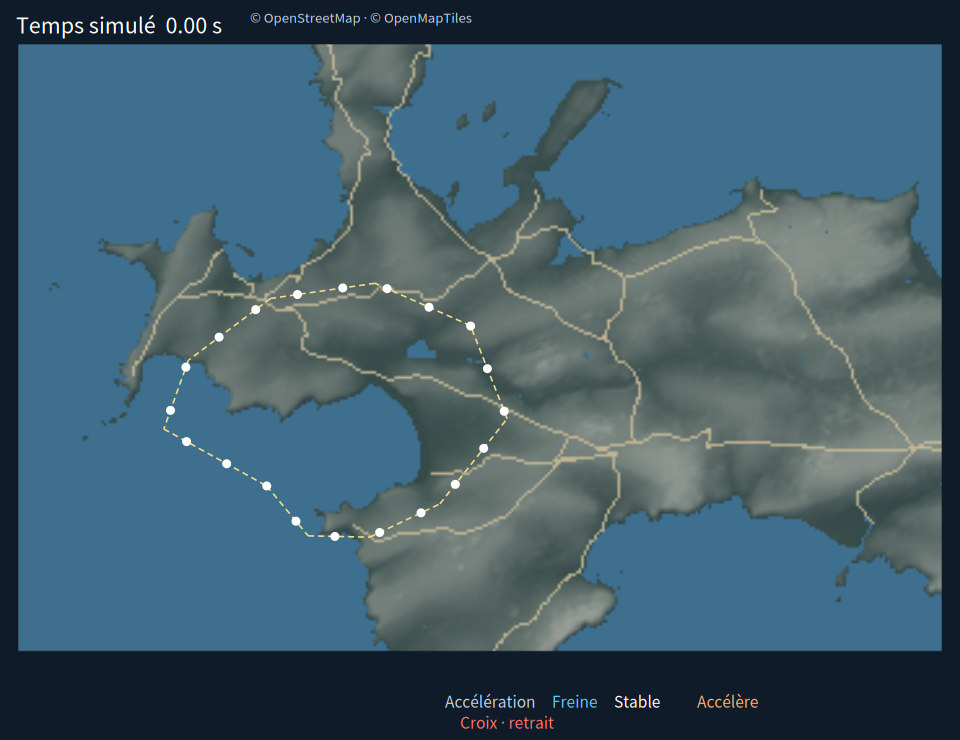
\includegraphics[width=.485\linewidth]{crozon-hillshade.jpg}\hfill
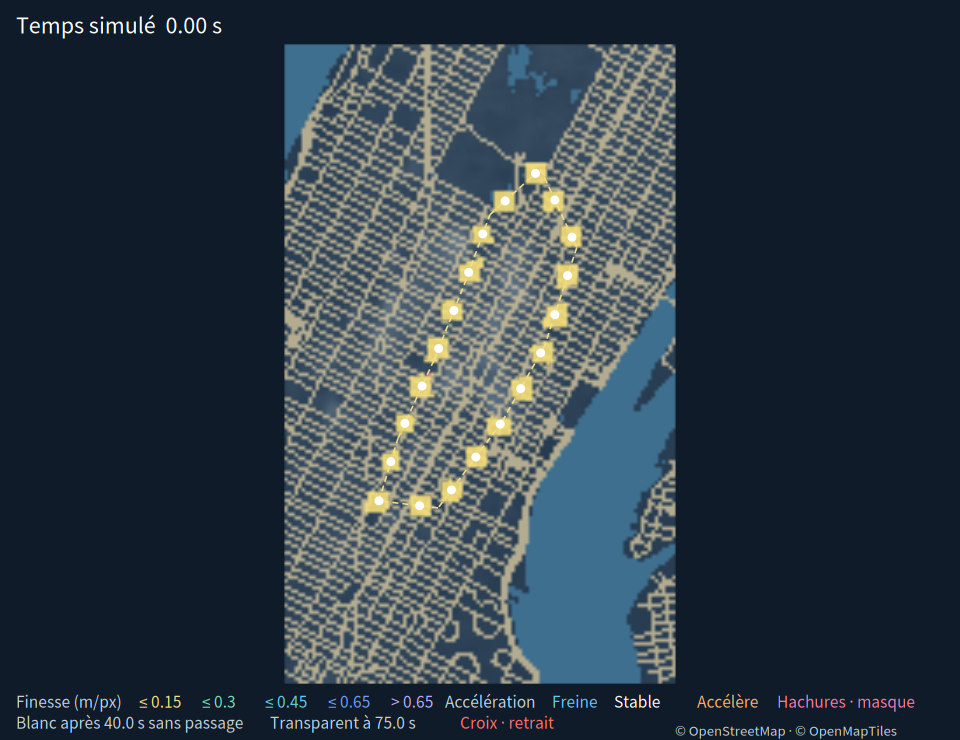
\includegraphics[width=.485\linewidth]{nyc-elevation.jpg}
\caption{Rejeux Roassal sur les grilles Copernicus, avec routes et eau issues d'OpenStreetMap. À gauche, ombrage du littoral de Crozon. À droite, altitude à Manhattan.}
\end{figure}

Les entrées de simulation sont lues au clic sur \ui{Simuler}. Les options d'affichage, de lecture et de CSV sont lues à chaque export ou rejeu. Vous pouvez recalculer la fraîcheur à une autre limite d'âge ou refaire une vidéo au ralenti à partir du même historique.

\section{Définir un terrain et un parcours}
\begin{enumerate}
\item Cliquez sur \ui{Dessiner sur la carte…}. Pour délimiter votre emprise, activez \ui{Emprise} et choisissez deux coins opposés. Un rectangle seul suffit à préparer le terrain.
\item Activez \ui{Point} et ajoutez les points de passage dans l'ordre. Pour importer les points par code, utilisez leurs coordonnées WGS84 longitude puis latitude. Trois sommets distincts suffisent à former une boucle. Cochez \ui{Enveloppe convexe} si le parcours doit suivre les sommets extérieurs calculés.
\item Cliquez sur \ui{Enregistrer le terrain…} et choisissez le nom, la source, la maille en mètres et la marge. Confirmez le dossier dans Pharo. \ui{Ouvrir un MNT…} recharge la grille et son tracé. Dans le navigateur, \ui{Enregistrer le tracé} produit un JSON autonome de l'emprise et des points.
\end{enumerate}

Une marge étend le MNT autour de l'emprise pour le rendu du champ optique. Une maille deux fois plus fine dans les deux directions représente environ quatre fois plus de cellules à emprise constante. Elle affine les bords de couverture et la représentation du relief si la source contient cette information. Le MNT discrétise chaque mesure sur une cellule rectangulaire. Le bord visible de l'empreinte est donc crénelé suivant la grille. Commencez avec un petit rectangle pour vérifier l'échelle avant un export fin.

\begin{tabularx}{\linewidth}{@{}lY@{}}
\toprule
Entrée de terrain & Usage \\
\midrule
Copernicus GLO-30 & Modèle de surface international avec téléchargement des dalles publiques et reprojection. Bâtiments et végétation sont représentés à la résolution de la source. \\
IGN ou USGS & Choix d'une source d'altitude locale dans sa zone de couverture. Renseignez au besoin un GeoTIFF de provenance connue qui couvre l'emprise et la marge. \\
GeoTIFF local & Découpez une source déjà téléchargée ou un raster produit par vos outils. Vérifiez son système de coordonnées et les zones sans données. \\
\bottomrule
\end{tabularx}

\textbf{Le fond de carte est un réglage d'affichage.} OpenStreetMap aide à placer les points dans le navigateur. Sur une grille préparée, \ui{Relief ombré} utilise l'ombrage calculé à partir des hauteurs. \ui{Altitude} colore ces hauteurs et \ui{Aucun} conserve les couches que vous activez. Les exemples embarqués combinent relief et géométries de littoral, d'eau et de routes. \ui{Plan IGN}, \ui{USGS Topo} et \ui{Sentinel-2 (mosaïque 2016)} utilisent leurs fonds externes dans le navigateur et en rendu. Les rasters d'affichage sont reprojetés dans le repère et l'emprise des observations. Plan IGN couvre la France, USGS Topo couvre les États-Unis et Sentinel-2 est mondial à la latitude des zones fournies. Les fonds Plan IGN et Sentinel-2 de Crozon et du Vercors ainsi que le fond USGS Topo de Manhattan sont disponibles hors ligne dans le rendu natif. Pour une nouvelle emprise, leur préparation demande Internet et GDAL. Les fonds externes du navigateur utilisent les tuiles en direct.

\begin{figure}[ht]
\centering
\begin{minipage}[t]{.32\linewidth}
\centering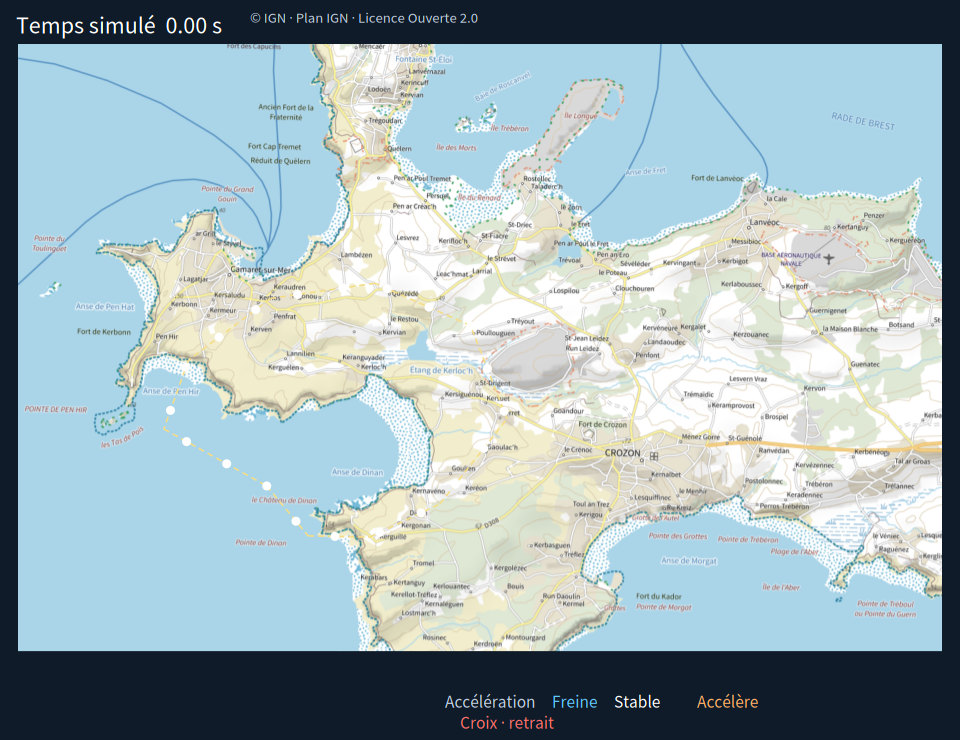
\includegraphics[width=\linewidth,height=37mm,keepaspectratio]{planIgn-crozon.jpg}\par
\small Plan IGN, Crozon\\© IGN
\end{minipage}
\begin{minipage}[t]{.32\linewidth}
\centering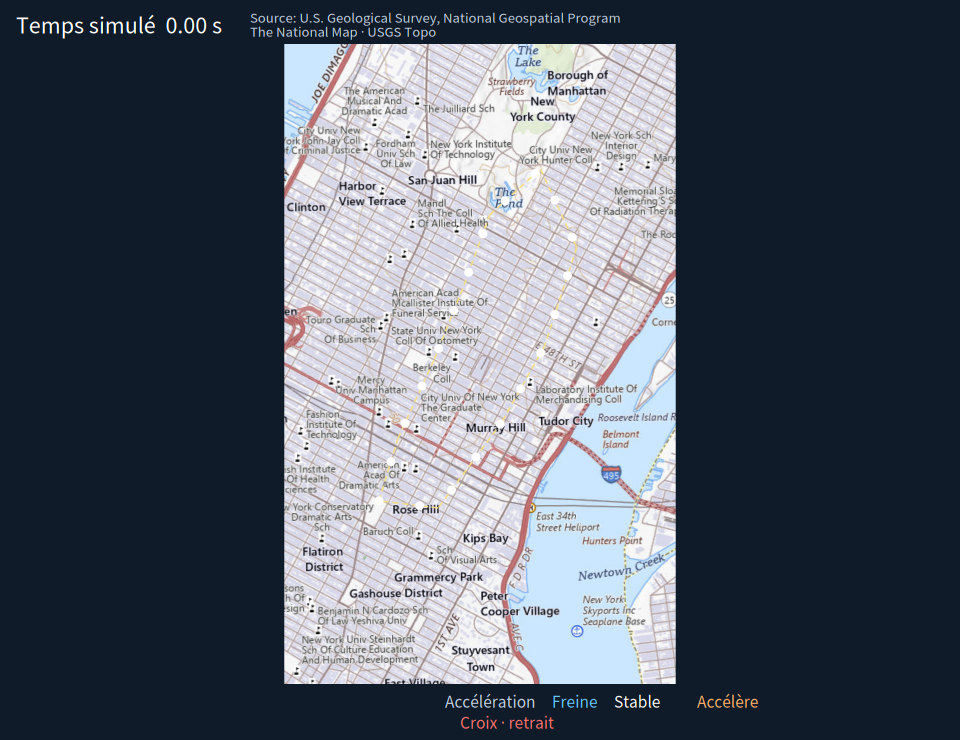
\includegraphics[width=\linewidth,height=37mm,keepaspectratio]{usgsTopo-nyc.jpg}\par
\small USGS Topo, Manhattan\\USGS The National Map
\end{minipage}
\begin{minipage}[t]{.32\linewidth}
\centering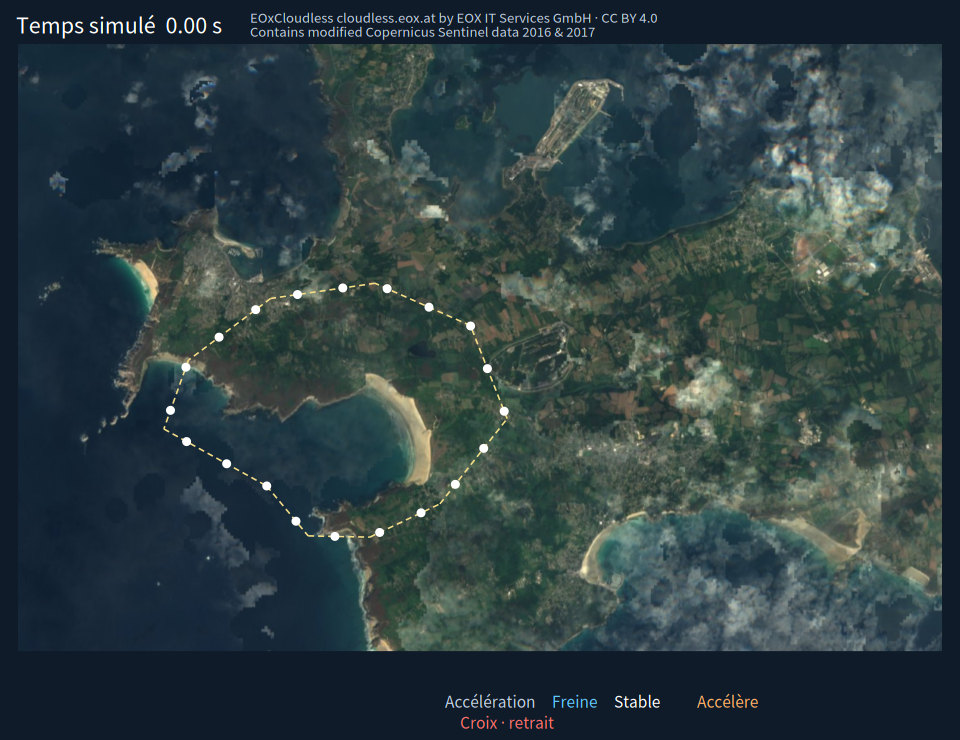
\includegraphics[width=\linewidth,height=37mm,keepaspectratio]{sentinel2-crozon.jpg}\par
\small Sentinel-2, Crozon\\EOX, CC BY 4.0
\end{minipage}
\caption{Images Roassal avec les trois fonds reprojetés et les tracés d'exemple. La mosaïque EOX contient des données Copernicus Sentinel modifiées de 2016–2017.}
\end{figure}

\begin{tabularx}{\linewidth}{@{}lrlY@{}}
\toprule
Exemple & Maille & Projection & Exercices \\
\midrule
Vercors & \multicolumn{2}{l}{grille livrée avec le rejeu} & Observer les zones masquées sur les versants et tester un changement de hauteur. \\
Crozon & 50 m & EPSG:32630 & Comparer mailles et lecture des falaises. \\
Manhattan & 30 m & EPSG:32618 & Vérifier l'alignement du tracé sur un plan urbain. \\
Détroit d'Ormuz & 250 m & EPSG:32640 & Examiner le relief et le littoral à l'échelle régionale sur un fond public archivé. \\
\bottomrule
\end{tabularx}

\section{Paramétrer la simulation et la perception}
\begin{tabularx}{\linewidth}{@{}p{.33\linewidth}Y@{}}
\toprule
Paramètre & Rôle \\
\midrule
Effectif, nombre et durée des tiks & Nombre initial de drones, horizon discret et conversion vers les secondes simulées. L'historique d'une exécution neuve contient l'état initial suivi des états produits. \\
Vitesses min, nominale, max & Entrées de la configuration en m/s. À l'intérieur du modèle macro, les commandes représentent un déplacement en m par tik. \\
Portée voisins & Distance de détection entre drones en mètres. Dans le modèle géométrique, la portée utilise la distance droite entre les positions. \\
Capture macro & Rayon en mètres d'arc devant et derrière le drone pour la mesure de couverture de la boucle. Une valeur nulle laisse la simulation de voisinage fonctionner. \\
Demi-angle gisement & Ouverture autour de l'axe local attendu, avant pour le successeur et arrière pour le prédécesseur. Agit sur les observations angulaires. \\
Poids des écarts & Gain entre 0 et 10 appliqué à l'erreur relative d'espacement dans la branche de correction des lois intégrées. La valeur historique est 2. \\
Objectif revisite, graine & Délai embarqué en secondes pour la troisième loi et graine de reproductibilité. L'indice ISSe permet de retrouver la graine du scénario historique. \\
\bottomrule
\end{tabularx}

Pour le voisin avant et le voisin arrière, la loi reçoit des écarts mesurés le long de la boucle. Une observation directe utilise la position du voisin dans la portée et donne l'écart d'arc. Une observation angulaire estime cet écart par l'intersection du gisement avec le parcours. Chaque rayon doit fournir une intersection admissible unique. Les coins, segments alignés ou intersections multiples peuvent rendre l'observation indisponible. Une loi intégrée conserve la vitesse si l'un des écarts manque.

\begin{tabularx}{\linewidth}{@{}lY@{}}
\toprule
Perception des voisins & Comportement \\
\midrule
Selon le scénario & Garde le modèle installé par l'exemple. À utiliser pour reproduire une référence historique. \\
Distance seule & Utilise une mesure directe disponible. \\
Gisement seul & Utilise l'écart reconstruit par le gisement, sous réserve du champ et de la géométrie. \\
Distance puis gisement & Essaie d'abord la distance, puis le gisement si la distance est indisponible. \\
\bottomrule
\end{tabularx}

\subsection{Lois de commande et délai de revisite}
Avec deux écarts disponibles, la correction se fonde sur
\[
e=\frac{g_{\text{avant}}-g_{\text{arrière}}}{\max(g_{\text{avant}},g_{\text{arrière}})}
\]
pour un dénominateur non nul. En dehors de la bande de sensibilité, la vitesse précédente est multipliée par $1 + w e$ avec le poids $w$. Les lois intégrées bornent la consigne. Dans la bande d'équilibre, les trois lois agissent différemment.

\begin{tabularx}{\linewidth}{@{}lY@{}}
\toprule
Loi & Dans la bande d'équilibre \\
\midrule
Capping & Applique le facteur \sel{pacingRate} à la vitesse courante, avec arrondi et bornes. Une flotte dont les écarts sont déjà équilibrés peut ainsi descendre à la vitesse minimale. \\
Capping révisé & Rapproche la vitesse de la nominale par le gain \sel{pacingRate}. \\
Capping avec revisite & Vise le maximum entre la vitesse nominale et le plus grand écart local divisé par le délai demandé. Applique le même rapprochement vers cette référence et les bornes de vitesse. \\
\bottomrule
\end{tabularx}

Dans \ui{Revisite}, \ui{Estimer le réglage courant} donne les ordres de grandeur $L/N$ et $L/(Nv)$ pour une boucle de longueur $L$ et $N$ drones régulièrement espacés. Si la vitesse requise est au-dessus du maximum, le réglage est hors d'atteinte dans cette approximation. La troisième loi utilise les deux observations locales et un délai embarqué parfois partagé par toute la flotte. Elle estime un intervalle de passage sur l'anneau. La fraîcheur d'une case du MNT dépend également du relief, du champ de la caméra et des passages effectifs.

\section{Lire et exporter une démonstration}
\begin{figure}[ht]
\centering
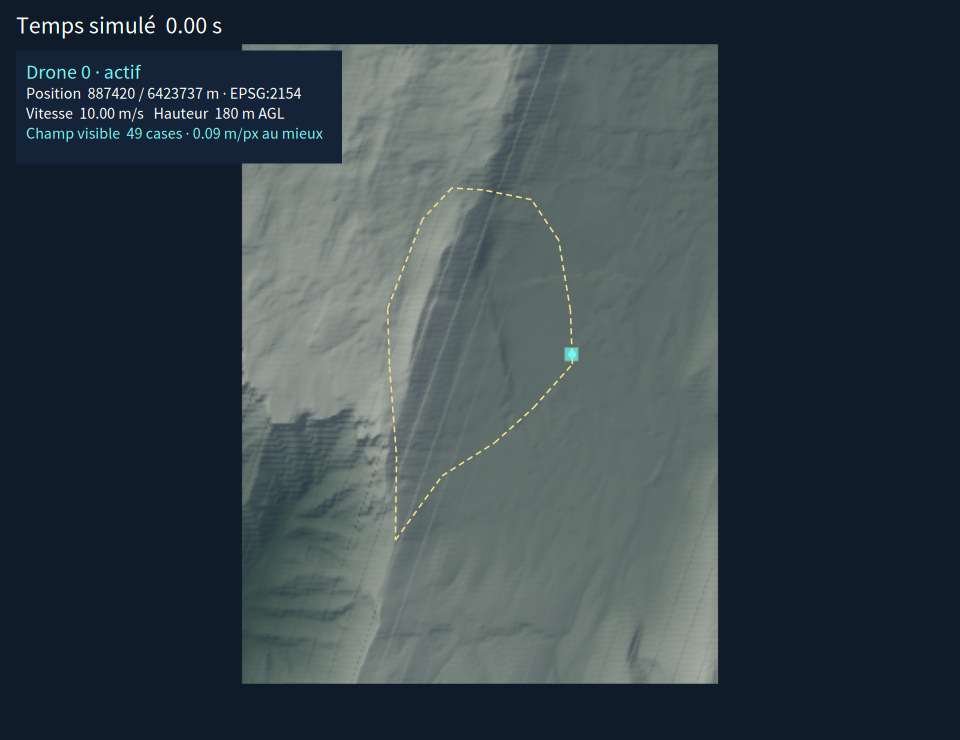
\includegraphics[width=.75\linewidth]{selection-drone.jpg}
\caption{Image de rejeu avec une incrustation de suivi et le champ d'un drone sur le relief.}
\end{figure}

\begin{tabularx}{\linewidth}{@{}p{.35\linewidth}Y@{}}
\toprule
Affichage & Effet \\
\midrule
Hauteur sol et champ optique & En mètres au-dessus du terrain sous le drone et en degrés. Sur un plan horizontal à incidence verticale, la largeur théorique vaut $2 h \tan(\theta/2)$. Le relief modifie la taille des zones visibles et la finesse au sol. \\
Couverture, masques, parcours & Affichez l'empreinte calculée et ses zones masquées par le relief. Décochez \ui{Afficher la couverture} et \ui{Hachurer les masques} pour isoler la flotte et son tracé. \\
Couleur des drones & \ui{Vitesse} compare la vitesse courante à la nominale. Par défaut, le bleu correspond à moins de 95\,\%, le blanc à 95–105\,\% et l'orange à plus de 105\,\%. \ui{Accélération} utilise la variation de vitesse par seconde et le seuil en m/s², avec freinage bleu, phase stable blanche et accélération orange. \ui{Uniforme} utilise une couleur commune. \\
Identifiants, statuts, retraits & Les identifiants et les statuts sont optionnels. Un retrait peut rester matérialisé à sa dernière position pendant la durée choisie. \\
Incrustation & Choisissez l'identifiant suivi et activez le surlignage de son champ pour associer au champ sa position projetée, sa vitesse, sa hauteur, le nombre de cases visibles et la meilleure finesse en m/px. \\
Blanc complet et effacement & L'information vieillit après le dernier passage. Elle blanchit jusqu'au premier seuil, puis devient transparente au second. Une nouvelle observation réinitialise l'âge. Placez l'effacement après le blanc complet. \\
\bottomrule
\end{tabularx}

Pour rendre une rupture de service lisible, choisissez le délai de blanc complet au voisinage du délai de revisite à l'équilibre et ajoutez une marge avant effacement. Comparez les mêmes bornes avant et après le retrait ou l'arrivée. Si la vitesse réelle est divisée par deux sur un segment, le délai de passage y double à espacement constant. Dans une flotte régulée, les écarts peuvent bouger en même temps. Le CSV optique montre l'effet net sur les cases fraîchement observées.

\textbf{Lecture à vitesse variable.} À $20\times$, 20 secondes simulées occupent une seconde de vidéo. \ui{Ralentir un intervalle de tiks} applique la vitesse ralentie dans l'intervalle choisi. \ui{Ralentir dans la zone GPS} l'applique quand un drone admissible entre dans le rectangle WGS84. Si les deux critères sont actifs, l'un suffit. Un pas d'images de 1 conserve chaque état à l'écran. Un pas plus grand réduit le volume des PNG. Le manifeste FFmpeg conserve les changements de cadence entre les images échantillonnées. Ce montage ne change pas l'âge simulé de l'information.

\section{Mesurer la qualité de service}
\begin{tabularx}{\linewidth}{@{}>{\raggedright\arraybackslash}p{.41\linewidth}Y@{}}
\toprule
Colonnes et panneaux & Lecture \\
\midrule
\sel{timeStep}, \sel{fleetSize}, \sel{avgSpeed} & Tik, effectif actif et déplacement moyen par tik. Divisez \sel{avgSpeed} par la durée du tik pour des m/s. \\
\sel{stdGap}, \sel{maxGap}, \sel{coverageRatio} & Dispersion et maximum des espacements en mètres d'arc, et couverture macro selon la capture. \\
\sel{directPerceptionRatio}, \sel{angularPerceptionRatio}, \sel{unobservablePerceptionRatio}, \sel{outOfRangePerceptionRatio} & Fraction des observations de voisinage dans chaque catégorie, avec erreur moyenne d'écart via \sel{avgGapEstimationError}. \\
\sel{opticalCoverageRatio}, \sel{freshCoverageRatio}, \sel{freshnessStatus} & Fraction de cases visibles à ce tik, fraction de cases d'âge inférieur ou égal au blanc complet, et verdict selon la cible choisie. Le dénominateur est le MNT ou la zone GPS de mesure. \\
\ui{Revisite} & Compare les deux derniers historiques. Le pire délai estimé à chaque tik combine le plus grand quotient local écart/vitesse. Le délai d'évaluation peut être modifié après simulation. \\
\bottomrule
\end{tabularx}

Exemple de contrat de lecture utilisable en CSV. Évaluez à chaque tik la fraction de cellules vues depuis au plus 40 s dans une zone GPS fixée et prenez comme objectif 75\,\%. Gardez ces seuils identiques pour toutes les variantes. \ui{Mesurer dans la zone GPS de Lecture} applique le rectangle à la métrique et s'active indépendamment du ralenti. Une variante peut améliorer l'espacement macro et laisser un versant masqué. Le verdict optique permet de constater cette différence.

\subsection{Interroger un historique en Pharo}
\sel{evaluateMetrics} retourne un \sel{MacroSimulatorMetricsHistory}. Pour une mission déjà simulée, sélectionnez un indicateur et un seuil adapté à la question, ici un espacement maximum de 800 m.

\begin{lstlisting}
| metriques trous premier |
metriques := simulateur evaluateMetrics.
trous := metriques intervalsOf: #maxGap
                   where: [ :ecart | ecart > 800 ].
premier := metriques firstTimeOf: #maxGap
                     where: [ :ecart | ecart > 800 ].
{ premier. trous } inspect.
\end{lstlisting}

Les bornes d'un intervalle sont des tiks inclusifs. Les requêtes \sel{longestDurationOf:where:} et \sel{totalDurationOf:where:} comptent des échantillons. Pour estimer la durée en secondes, multipliez par la période du tik si chaque échantillon représente l'intervalle qui le suit. Les extracteurs de convergence et de stabilisation permettent de préciser une cible, une tolérance et une durée de confirmation. Dans la console, \sel{minGap}, \sel{avgGap}, \sel{maxUncoveredGap}, \sel{totalUncoveredLength} et les statistiques de vitesse complètent les colonnes de base. Une erreur d'estimation peut valoir zéro quand aucune observation n'est disponible. Vérifiez les ratios d'observation avant de l'interpréter.

\clearpage
\section{Lancer les expériences depuis un Terminal}
\label{sec:experiences}
Les fichiers sous \sel{exemples/} donnent des configurations relisibles. Les modes \sel{run}, \sel{compare}, \sel{video} et \sel{terrain} utilisent la même classe de paramètres depuis une image Pharo sans interface. Exécutez les commandes depuis le dossier de l'atelier. Adaptez le chemin de la VM et celui de l'image en fonction de l'installation.

\begin{lstlisting}
bash lancer-lot.sh "$VM_PHARO" "$IMAGE_PHARO" \
  exemples/legacy-sose.json ./resultats/legacy run

bash lancer-lot.sh "$VM_PHARO" "$IMAGE_PHARO" \
  exemples/comparaison-synthetique.json ./resultats/comparaison compare
\end{lstlisting}

Avec le lanceur de l'image installée, vous pouvez aussi utiliser ce raccourci.

\begin{lstlisting}
atelier="$HOME/sose-propre"
"$atelier/lancer.sh" lot \
  "$atelier/exemples/comparaison-synthetique.json" \
  "$atelier/resultats/comparaison" compare
\end{lstlisting}

Le fichier \sel{legacy-sose.json} rejoue le modèle SoSe historique. Conservez le mode de perception du scénario, les événements et la graine pour comparer une version de l'image à une autre. Testez les lois et hypothèses alternatives avec \sel{comparaison-synthetique.json}, où le parcours est défini en géométrie plane. La boucle fournit les intersections nécessaires à la reconstruction angulaire, y compris en l'absence de polygone WGS84.

\begin{lstlisting}
| options sortie |
options := SoSeAtelierParameters exampleComparison.
options
    at: #distanceWeight put: 2.0;
    at: #bearingHalfAngle put: 180.0.
options writeTo: FileLocator workingDirectory / 'comparaison.json'.
options := SoSeAtelierParameters readFrom:
    FileLocator workingDirectory / 'comparaison.json'.
sortie := FileLocator workingDirectory / 'comparaison'.
options runComparisonInto: sortie.
\end{lstlisting}

Pour utiliser la même configuration sur un terrain, sélectionnez un exemple avec \sel{terrainExample:} ou associez un MNT avec \sel{terrainDirectory:} et un parcours via \sel{path:}. Les \sel{Point} d'un parcours WGS84 utilisent `longitude@latitude'. Le mode \sel{video} requiert un terrain avec une grille préparée. Le JSON de paramètres utilise le format \sel{sose-atelier-parameters}, version 1. Un chemin de terrain relatif est résolu depuis le dossier du fichier JSON. L'exemple synthétique sert à comparer les lois avec un protocole stable. Simulez une fois par variante et comparez le maximum et l'écart-type des espacements, la vitesse et les parts d'observations refusées. Gardez constantes la graine, la portée, la cadence d'intégration et les vitesses bornes lorsque vous isolez l'effet d'un paramètre.

\subsection{Préparer une grille et lancer une vidéo}
Le fichier \sel{exemples/crozon-video.json} rejoue la grille côtière embarquée, avec un intervalle ralenti entre les tiks 10 et 15. Il sert à vérifier FFmpeg et le rendu avant de générer un nouveau terrain.

\begin{lstlisting}
bash lancer-lot.sh "$VM_PHARO" "$IMAGE_PHARO" \
  exemples/crozon-video.json ./resultats/crozon video
\end{lstlisting}

Depuis un Playground, fournissez la boîte géographique sous la forme ouest, sud, est, nord. Dans cet exemple, les quatre points du parcours sont conservés avec la grille. Retirez l'appel \sel{path:} pour calculer la grille avant de tracer le parcours.

\Needspace{14\baselineskip}
\begin{lstlisting}
| p destination |
p := SoSeAtelierParameters new
    terrainBounds: #(-4.56 48.22 -4.44 48.32);
    path: { -4.54 @ 48.25. -4.47 @ 48.25.
            -4.46 @ 48.28. -4.50 @ 48.30 };
    gridStep: 50;
    terrainMargin: 300;
    terrainSource: #copernicus;
    heightAboveGround: 150;
    fieldOfView: 55;
    yourself.
destination := FileLocator home / 'crozon-mission'.
p prepareTerrainInto: destination.
p writeTo: FileLocator home / 'crozon-mission.json'.
\end{lstlisting}

\begin{lstlisting}
bash lancer-lot.sh "$VM_PHARO" "$IMAGE_PHARO" \
  "$HOME/crozon-mission.json" ./resultats/crozon video
\end{lstlisting}

Pour préparer la grille directement depuis un JSON, utilisez le mode \sel{terrain}. Le dossier de destination devient le dossier de MNT, avec un fichier \sel{parametres.json} prêt à relire. Pour un rendu du jeu livré en un raccourci, \sel{terrainExample: 'crozon'} charge la grille et le tracé fournis, et \sel{displayAt: \#background put: \#planIgn} sélectionne le fond. \sel{playbackAt:put:} ajoute les options de lecture \sel{normalRate}, \sel{slowRate}, \sel{stride}, \sel{interval} ou \sel{hotspot}. \sel{metricZone:} définit le rectangle de mesure optique indépendamment du ralenti.

\clearpage
\subsection{Lire les résultats d'une comparaison}
Les paramètres de voisinage et le poids des écarts répondent à deux questions distinctes. Le poids règle l'intensité de la correction quand les écarts observés sont déséquilibrés. Le demi-angle de gisement règle où les observations angulaires peuvent être produites. Les métriques de perception montrent combien de fois la loi a effectivement reçu les entrées nécessaires. Une comparaison des trajectoires seule laisse cette information implicite.

\begin{figure}[ht]
\centering
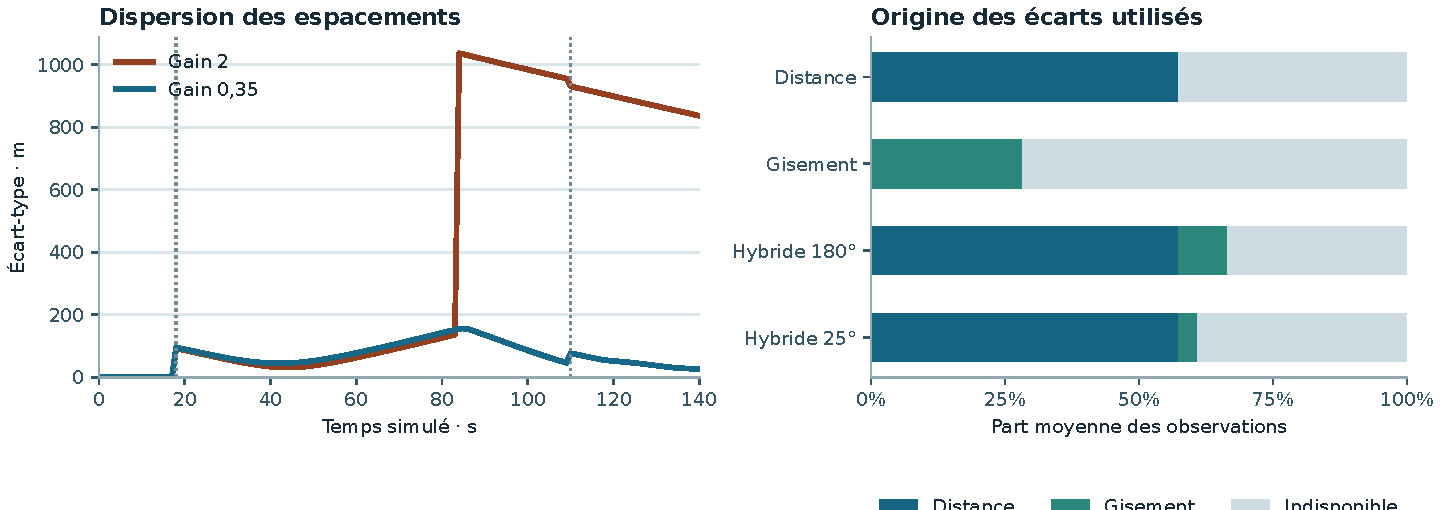
\includegraphics[width=\linewidth]{comparaison.pdf}
\caption{Résultats de Pharo 14 sur la boucle synthétique de 4 km avec 12 drones au départ et un tik de 1 s. Pointillés aux tiks 18 et 110 pour le retrait et l'entrée. Le retrait des mesures de distance aux tiks 25–84 et du gisement aux tiks 45–69 est commun à tout le lot.}
\end{figure}

Le lot écrit un dossier par variante avec son JSON et sa série \sel{simulation-timeseries.csv}, et un tableau \sel{comparaison.csv}. Les résultats livrés sous \path{exemples/resultats-reference/} servent à vérifier le rejeu. Dans le jeu perturbé, le gain 0,35 réduit l'écart-type final de 837 m à 27 m sur l'hybride. Le délai de revisite estimé au dernier état passe de 229,1 s à 65,5 s. Le demi-angle de 25° fait baisser la part des observations angulaires de 9,0\,\% à 3,4\,\% dans l'hybride. Cette ouverture n'a pas changé la part des observations directes. Les valeurs décrivent cette trajectoire, cette graine et ces indisponibilités.

Avec le même retrait et la même entrée, la variante \ui{Capping avec revisite} dépasse encore l'objectif de 32 s au dernier état. La boucle géométrique contient des mesures d'espacement et une estimation de revisite sur l'anneau.

\textbf{Lois à l'équilibre.} Pour isoler l'effet du délai embarqué, exécutez le mode \sel{compare} avec \sel{exemples/revisite-equilibre.json}. Ce jeu garde les 12 drones initialement espacés de 333 m et les observations directes disponibles pendant 140 tiks. Le tableau reprend les résultats finaux pour les trois lois en mode hybride.

\begin{tabularx}{\linewidth}{@{}Yrrr@{}}
\toprule
Variante & Vitesse moyenne & Délai estimé & États au-delà de 32 s \\
\midrule
Capping & 5,00 m/s & 66,67 s & 141 \\
Capping révisé & 10,00 m/s & 33,33 s & 141 \\
Capping avec revisite & 10,42 m/s & 32,00 s & 8 \\
\bottomrule
\end{tabularx}

Pour une comparaison optique, fixez la loi et le scénario, rejouez l'historique à deux hauteurs et exportez \sel{opticalCoverageRatio} et \sel{freshCoverageRatio} sur la même grille. Pour comparer le retour de service après un retrait et un renfort, figez les réglages d'affichage, activez les retraits et ralentissez une fenêtre centrée sur chaque événement. Comparez aussi dans le CSV le délai entre l'événement et le retour au-dessus de la cible sur la même zone.


\clearpage
\part{Intégrer et maintenir}

\section{Reconstruire une image Pharo 14}
Téléchargez une image Pharo 14 vierge et une VM correspondant à l'architecture de la machine. Placez-vous à la racine du kit extrait. Le troisième argument doit désigner un nouveau dossier. Sur macOS, passez le chemin du binaire \sel{Pharo} sous \sel{Pharo.app/Contents/MacOS}.

\begin{lstlisting}
bash installer.sh "/chemin/vers/pharo" \
  "/chemin/vers/Pharo 14.image" "$HOME/sose-propre"

"$HOME/sose-propre/lancer.sh"
\end{lstlisting}

L'installateur importe le socle FullApp figé et NeoCSV embarqués, charge les paquets Tonel de l'atelier, associe les ressources et vérifie l'image. Le répertoire résultat contient \sel{SoSe-Atelier.image}, son lanceur et un dépôt Git local dans \sel{atelier/}. Examinez \sel{provenance.txt} et \sel{verification.txt} pour retrouver les versions et les contrôles. Le socle livré fonctionne sans accès à un dépôt distant à l'installation. Les ressources cartographiques externes restent soumises à la disponibilité des fournisseurs.

Pour utiliser une autre révision FullApp, ajoutez \sel{--fullapp-clone CHEMIN} ou \sel{--fullapp-url URL}, avec \sel{--ref REF} pour figer la révision. Pour préparer une publication, \sel{--clone-publication URL} crée un clone séparé dans \sel{publication/}, prépare les sources sur la branche de travail \sel{atelier-sose} et laisse la révision et l'envoi à l'utilisateur. L'installation locale reste utile pour comparer les modifications de cette branche à l'état livré.

\begin{lstlisting}
git -C "$HOME/sose-propre/atelier" status
git -C "$HOME/sose-propre/publication" diff --cached --stat
\end{lstlisting}

\subsection{Dépendances par usage}
\begin{tabularx}{\linewidth}{@{}lY@{}}
\toprule
Usage & Dépendances \\
\midrule
Installation de référence & Git, Bash, VM et image Pharo 14. Le profil charge les classes FullApp nécessaires, NeoCSV et les services terrain. Il utilise Spec et Roassal de l'image Pharo 14 de départ. \\
Simulation et CSV & L'image installée et les fichiers de paramètres. Une comparaison sur boucle synthétique fournit son parcours sans téléchargement. \\
Terrain fourni & Les ressources locales de l'atelier. Elles comprennent les données des exemples. \\
MNT et fonds externes & GDAL dans le \sel{PATH}. Copernicus requiert \sel{curl}, \sel{gdalbuildvrt} et un accès aux dalles publiques. Les fonds externes nécessitent un accès à leur service. \\
Vidéo MP4 & FFmpeg dans le \sel{PATH}, avec l'encodeur \sel{libx264}. \\
Carte et 3D Web & Un navigateur récent. L'aperçu 3D utilise WebGL. \\
Documentation & LaTeX avec TikZ, \sel{listings} et \sel{hyperref}, pour recompiler le PDF. \\
\bottomrule
\end{tabularx}

Sur macOS Intel, si Homebrew ne propose pas une version de GDAL installable, utilisez les paquets \sel{osx-64} disponibles pour votre version de macOS dans Conda. Le nom du paquet est \sel{gdal}. Lancez ensuite l'atelier depuis le même Terminal pour qu'il hérite du \sel{PATH}.

\begin{lstlisting}
conda create -n sose-gdal --override-channels -c conda-forge gdal
conda activate sose-gdal
gdalinfo --version
gdalwarp --version
gdalbuildvrt --version
ffmpeg -version
"$HOME/sose-propre/lancer.sh"
\end{lstlisting}

Pour faire évoluer les paquets depuis Pharo, ajoutez le dépôt local dans Iceberg. Le fichier \sel{.project} place les paquets sous \sel{src}. Les changements de méthodes sont exportés en Tonel quand vous les commitez dans ce dépôt. Renouvelez une reconstruction sur image vierge pour vérifier le chargement à partir des seuls fichiers.

La référence de construction est \sel{guide-atelier.tex}. Depuis le dossier \sel{documentation}, la commande \sel{latexmk -pdf guide-atelier.tex} régénère ce document et ses diagrammes TikZ.


\section{Flux des classes et points d'extension}
\begin{center}
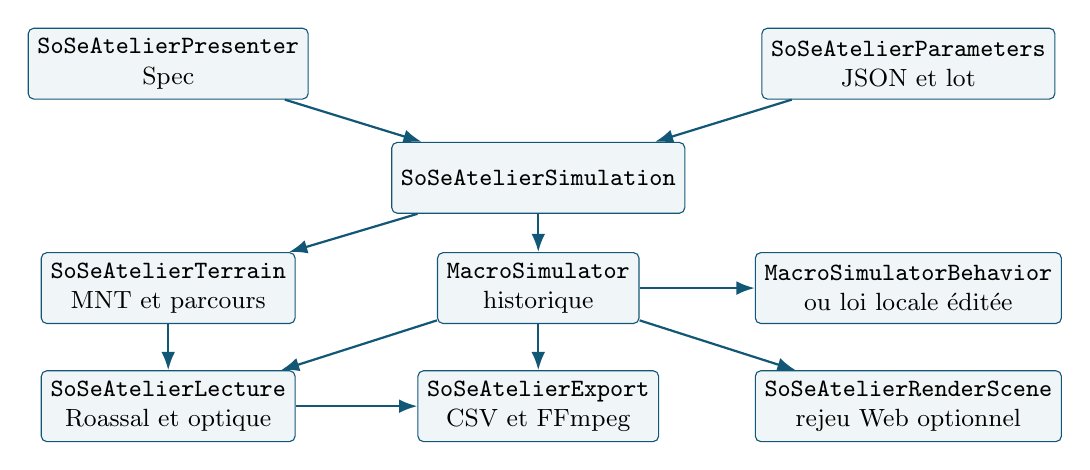
\begin{tikzpicture}[
every node/.style={draw=Bleu,rounded corners=2pt,minimum height=9mm,align=center,fill=Papier,font=\small},
edge/.style={-Latex,thick,draw=Bleu},x=1cm,y=1cm]
\node (gui) at (-4.7,0) {\sel{SoSeAtelierPresenter}\\Spec};
\node (cli) at (4.7,0) {\sel{SoSeAtelierParameters}\\JSON et lot};
\node (sim) at (0,-1.45) {\sel{SoSeAtelierSimulation}};
\node (terrain) at (-4.7,-2.85) {\sel{SoSeAtelierTerrain}\\MNT et parcours};
\node (macro) at (0,-2.85) {\sel{MacroSimulator}\\historique};
\node (law) at (4.7,-2.85) {\sel{MacroSimulatorBehavior}\\ou loi locale éditée};
\node (lecture) at (-4.7,-4.35) {\sel{SoSeAtelierLecture}\\Roassal et optique};
\node (export) at (0,-4.35) {\sel{SoSeAtelierExport}\\CSV et FFmpeg};
\node (web) at (4.7,-4.35) {\sel{SoSeAtelierRenderScene}\\rejeu Web optionnel};
\draw[edge] (gui) -- (sim);
\draw[edge] (cli) -- (sim);
\draw[edge] (sim) -- (macro);
\draw[edge] (sim) -- (terrain);
\draw[edge] (macro) -- (law);
\draw[edge] (terrain) -- (lecture);
\draw[edge] (macro) -- (lecture);
\draw[edge] (macro) -- (export);
\draw[edge] (macro) -- (web);
\draw[edge] (lecture) -- (export);
\end{tikzpicture}
\end{center}

\begin{tabularx}{\linewidth}{@{}>{\raggedright\arraybackslash}p{.39\linewidth}Y@{}}
\toprule
Service & Contrat \\
\midrule
\sel{SoSeAtelierMapPlan}, \sel{SoSeAtelierMapServer} & Échangent l'emprise et les points WGS84 entre le navigateur local et Spec. \sel{SoSeAtelierTerrain} raccorde les projections, la préparation GDAL et le rejeu. \\
\sel{SoSeAtelierResources} & Résout les chemins des pages, exemples et terrains. Reliez-le à la racine de l'atelier si vous déplacez le dossier. \\
\sel{SoSeAtelierCommandLaw}, \sel{SoSeAtelierLocalInput} & Conservent la source et les données nécessaires à une décision locale. Un éditeur d'équations pourra produire un bloc qui respecte le même contrat d'entrée. \\
\sel{SoSeAtelierMissionFile} & Sauve ou recharge la mission de l'interface avec son scénario, son tracé, son état de réglage et son catalogue. \\
\sel{SoSeAtelierRevisitRun} & Analyse un historique existant selon le délai de revisite testé. \\
\bottomrule
\end{tabularx}

\subsection{Ajouter une loi et un scénario}
Dans \ui{Commande}, \ui{Nouvelle} crée un bloc, \ui{Dupliquer} permet de partir d'une loi existante et \ui{Utiliser} le sélectionne pour la simulation. Le bloc reçoit un \sel{SoSeAtelierLocalInput}. Il renvoie la consigne de déplacement en m/tik. La structure expose \sel{gapAhead}, \sel{gapBehind}, \sel{hasBothGaps}, \sel{relativeGapError}, \sel{currentSpeed}, \sel{secondsPerTick} et \sel{revisitTargetSeconds}. L'entrée contient les mesures ou estimations effectivement accessibles au drone à ce tik.

\begin{lstlisting}
[ :local |
    local hasBothGaps
        ifTrue: [
            local currentSpeed
                + (local relativeGapError * local secondsPerTick) ]
        ifFalse: [ local currentSpeed ] ]
\end{lstlisting}

L'éditeur de scénarios accepte un bloc à un argument \sel{[ :atelier | \ldots ]} ou une méthode historique de \sel{MacroSimulatorExample class}. Pour rendre l'historique accessible à Roassal et aux exporteurs de l'atelier, retournez le \sel{MacroSimulator} exécuté. Placez l'initialisation des perceptions avant le premier mouvement. Pour comparer plusieurs stratégies de retrait ou d'entrée, utilisez une graine explicite, programmez vos événements dans le scénario, exécutez un horizon borné et gardez les mêmes conditions de départ. La courbe d'effectif et les métriques doivent être interprétées avec le journal des changements de flotte.

\subsection{Préserver les expériences historiques}
Le menu donne accès à \ui{SoSe historique}, \ui{SoSe paramétrable} et \ui{ISSe historique}. \ui{SoSe historique} appelle \sel{FullAppMacroReplay soSe}. \ui{SoSe paramétrable} reprend le scénario à événements sur un anneau de 10 km avec des réglages de simulation accessibles. \sel{FullAppMacroReplay isSeWithSeedIndex: 10} demande un scénario ISSe par son indice. Les campagnes accessibles dans \sel{MacroSimulatorExample class} peuvent produire leurs propres métriques ou exports. Après intégration, comparez les tiks, l'effectif et les séries historiques avec vos références avant d'attribuer un changement à une loi. Les méthodes \sel{run:} et \sel{runSingleUpdate:} ont des cadences historiques distinctes. La seconde fait un déplacement par tik et sert aux comparaisons géométriques indiquées ici.

\begin{lstlisting}
| simulateur metriques |
simulateur := FullAppMacroReplay soSe.
metriques := simulateur evaluateMetrics.
metriques last inspect.
\end{lstlisting}

Pour une campagne exportée via \sel{MacroExporter}, conservez les noms d'extracteurs et de colonnes déjà publiés. Les rapports optiques sont calculés dans le rejeu à partir de l'historique, de la grille, de l'âge et des paramètres d'affichage. Dans un rendu Pharo personnalisé, \sel{PerceptionMissionView} accepte trois \sel{movementColors}, deux \sel{speedRatioLimits}, cinq \sel{coverageColors} et quatre \sel{gsdLimits} croissants en m/px. Ceux-ci s'appliquent à la palette et aux classes de finesse. Le formulaire d'affichage règle le mode et le seuil d'accélération. Le couplage avec une classe de simulation existante se fait par son historique et ses instantanés d'état.

\subsection{Tracer la provenance d'un terrain et d'un résultat}
Une grille réutilisable comprend \sel{terrain.json}, \sel{mnt.csv}, \sel{emprise.geojson} et, pour une mission dessinée, \sel{trace-sose.json}. Le descripteur de grille donne \sel{crs}, \sel{topLeft}, \sel{cellSize}, \sel{columns} et \sel{rows}. Le fond associé suit la projection et l'emprise de la grille. Un fond externe peut être calculé à une résolution d'affichage distincte de la maille d'altitude. Sauvez le GeoTIFF d'origine ou son URL avec l'attribution, la date, le SCR et le pas retenu pour le rééchantillonnage.

Pour partager une expérience, versionnez les sources Tonel, le JSON des paramètres, les points, les grilles dont la licence autorise la redistribution et un relevé de provenance. Les images Pharo, fichiers \sel{.changes}, caches cartographiques et séries de PNG sont des sorties de travail. Sur Git, utilisez des ressources séparées pour les gros fichiers selon la politique de votre dépôt. Conservez l'identifiant de révision FullApp inscrit par l'installation, la graine, le mode de voisinage et la cadence d'intégration près du CSV et de la vidéo.

\section{Rejouer dans le navigateur}
Après \ui{Simuler}, cliquez sur \ui{Rejouer en 3D}. La scène reprend la hauteur au-dessus du sol et le pas de lecture. Fermer la fenêtre de l'atelier arrête le serveur de cette session.

Le service de dessin prépare l'emprise et les points de passage. Un service distinct de rejeu 3D ouvre une session locale à partir d'un historique existant. Le navigateur reçoit une description de scène JSON et affiche les positions sur une grille de relief, avec une boucle synthétique quand aucun terrain n'est fourni. Le visualiseur Three.js embarqué fournit une caméra orbitale et une vitesse de rejeu réglable. Roassal fournit les couches cartographiques, les observations optiques et les exports PNG et MP4.

\begin{lstlisting}
| scene serveur |
scene := SoSeAtelierRenderScene
    history: simulateur history
    tickSeconds: 1
    terrain: nil
    heightAboveGround: 180
    stride: 10.
serveur := SoSeAtelierRenderServer on: scene.
serveur open.
\end{lstlisting}

Conservez la référence au serveur pour appeler \sel{serveur stop}. Dans une mission géoréférencée, transmettez une instance de \sel{SoSeAtelierTerrain} et la durée de tik réellement utilisée par la simulation. \sel{scene writeTo:} conserve une scène versionnée pour le rejeu.

\begin{figure}[ht]
\centering
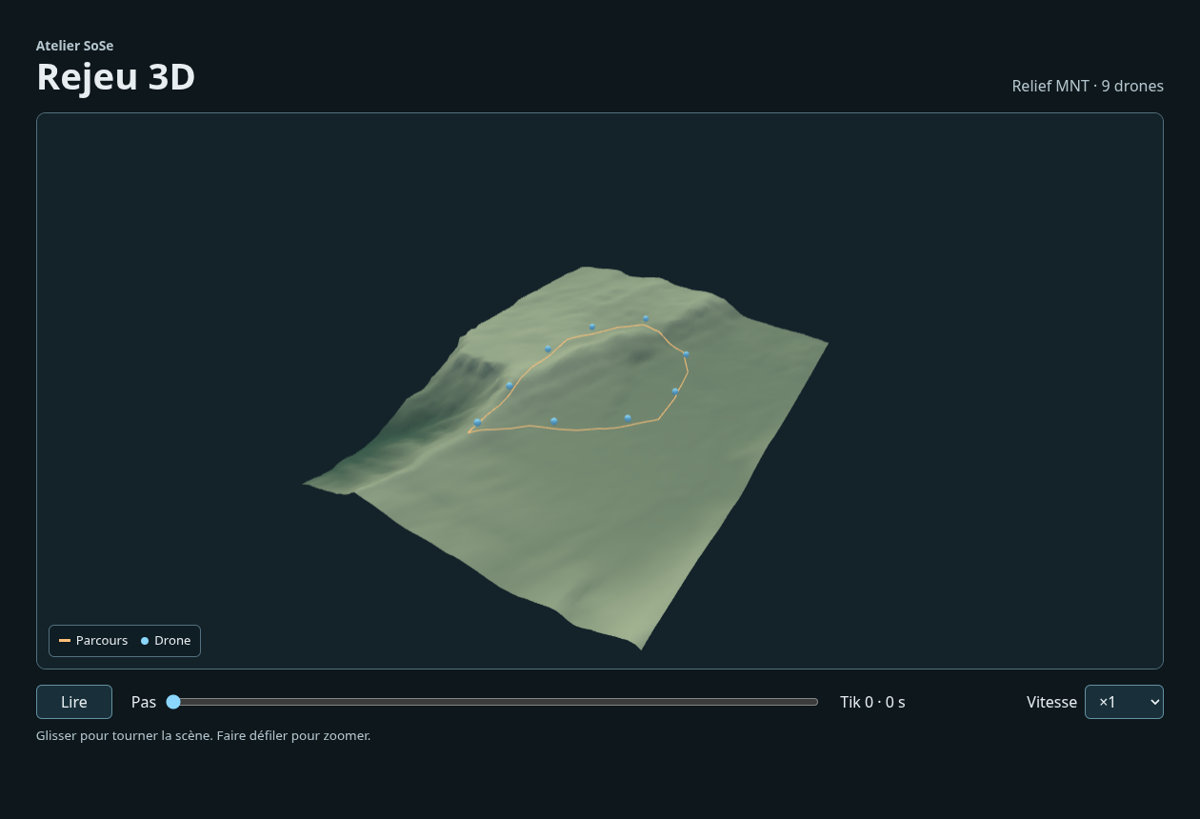
\includegraphics[width=.65\linewidth,height=51mm,keepaspectratio]{rejeu-web.jpg}
\caption{Rejeu Web en 3D d'un historique simulé sur le relief du Vercors. Le navigateur affiche le tracé et la position des drones aux états enregistrés.}
\end{figure}


\section{Sources cartographiques}
{\small
\textbf{Altitudes.} Produced using Copernicus WorldDEM-30 © DLR e.V. 2010–2014 and © Airbus Defence and Space GmbH 2014–2018 provided under COPERNICUS by the European Union and ESA; all rights reserved. \href{https://registry.opendata.aws/copernicus-dem/}{Copernicus DEM}.

\textbf{Fonds.} Eau et routes © OpenStreetMap contributors et © OpenMapTiles, via OpenFreeMap. Plan IGN © IGN. USGS The National Map. Sentinel-2 cloudless EOX, contient des données Copernicus Sentinel modifiées de 2016–2017, CC BY 4.0. \href{https://www.openstreetmap.org/copyright}{OpenStreetMap}. \href{https://openmaptiles.org/}{OpenMapTiles}. \href{https://openfreemap.org/}{OpenFreeMap}. \href{https://geoservices.ign.fr/services-web-experts-cartes}{IGN}. \href{https://www.usgs.gov/programs/national-geospatial-program/national-map}{USGS}. \href{https://s2maps.eu/}{EOX}.
\par}
\end{document}
